

\documentclass{beamer}
\usetheme{Berlin}
\usecolortheme{default}

\usepackage{cmap}                   % поиск в PDF
\usepackage{braket}
\usepackage[T2A]{fontenc}           % кодировка
\usepackage{mathtext}               % русские буквы в формулах
\usepackage[utf8]{inputenc}         % кодировка исходного текста
\usepackage[english,russian]{babel} % локализация и переносы
\usepackage{multimedia}             % вставка видео
\setbeamertemplate{caption}[numbered] % нумерование иллюстраций

\title{Реализация квантового компьютера на ионной ловушке}
\subtitle{Вопрос по выбору к ГКЭ, январь 2023}
\author{Талашкевич Даниил Б01-008}
\institute{Московский физико-технический институт}
\date{}

\newenvironment{comment}{}{}


% TODO:
% 1) Добавить формулы DONE
% 2) Исправить и добавить описание процесса
%    Инициализации
% 3) Добавить описание измерений
% 4) Проверить всю презентацию на ошибки

\begin{document}
    
    \begin{frame}
        \titlepage
    \end{frame}

    \begin{frame}{Содержание}

        \begin{itemize}

            \item Введение в квантовые вычисления
            
            \item Принцип работы ионной ловушки

                \begin{itemize}
                    \item{Захват иона}
                    \item{Доплеровское охлаждение}
                \end{itemize}

            \item Кубит на ионной ловушке

                \begin{itemize}
                    \item{Физическая реализация кубита}
                    \item{Приготовление начального состояния}
                    \item{Измерение конечного результата}
                \end{itemize}
      
        \end{itemize}            
        \end{frame}
	
	\begin{frame}{Введение в квантовые вычисления}
		Классический бит: $0$ или $1$ - два состояния.
		\vspace{3mm}
		
		Квантовый бит: $\ket{\psi} = \alpha\ket{0} + \beta\ket{1}$, $\alpha,\beta \in \mathbb{C}$, $|\alpha|^2 + |\beta|^2 = 1$ - бесконечно много состояний?
		\vspace{3mm}
		
		Представление на сфере Блоха: $\ket{\psi} = e^{i\gamma}\left(  \cos{\frac{\theta}{2}}\ket{0}+e^{i\phi}\sin{\frac{\theta}{2}} \ket{1}  \right) \sim \cos{\frac{\theta}{2}}\ket{0}+e^{i\phi}\sin{\frac{\theta}{2}} \ket{1} $,
		
		где $\gamma, \theta$ и $\phi$ - действительные числа.
	\end{frame}
	
	\begin{frame}{Введение в квантовые вычисления}
		
		\begin{figure}[]
			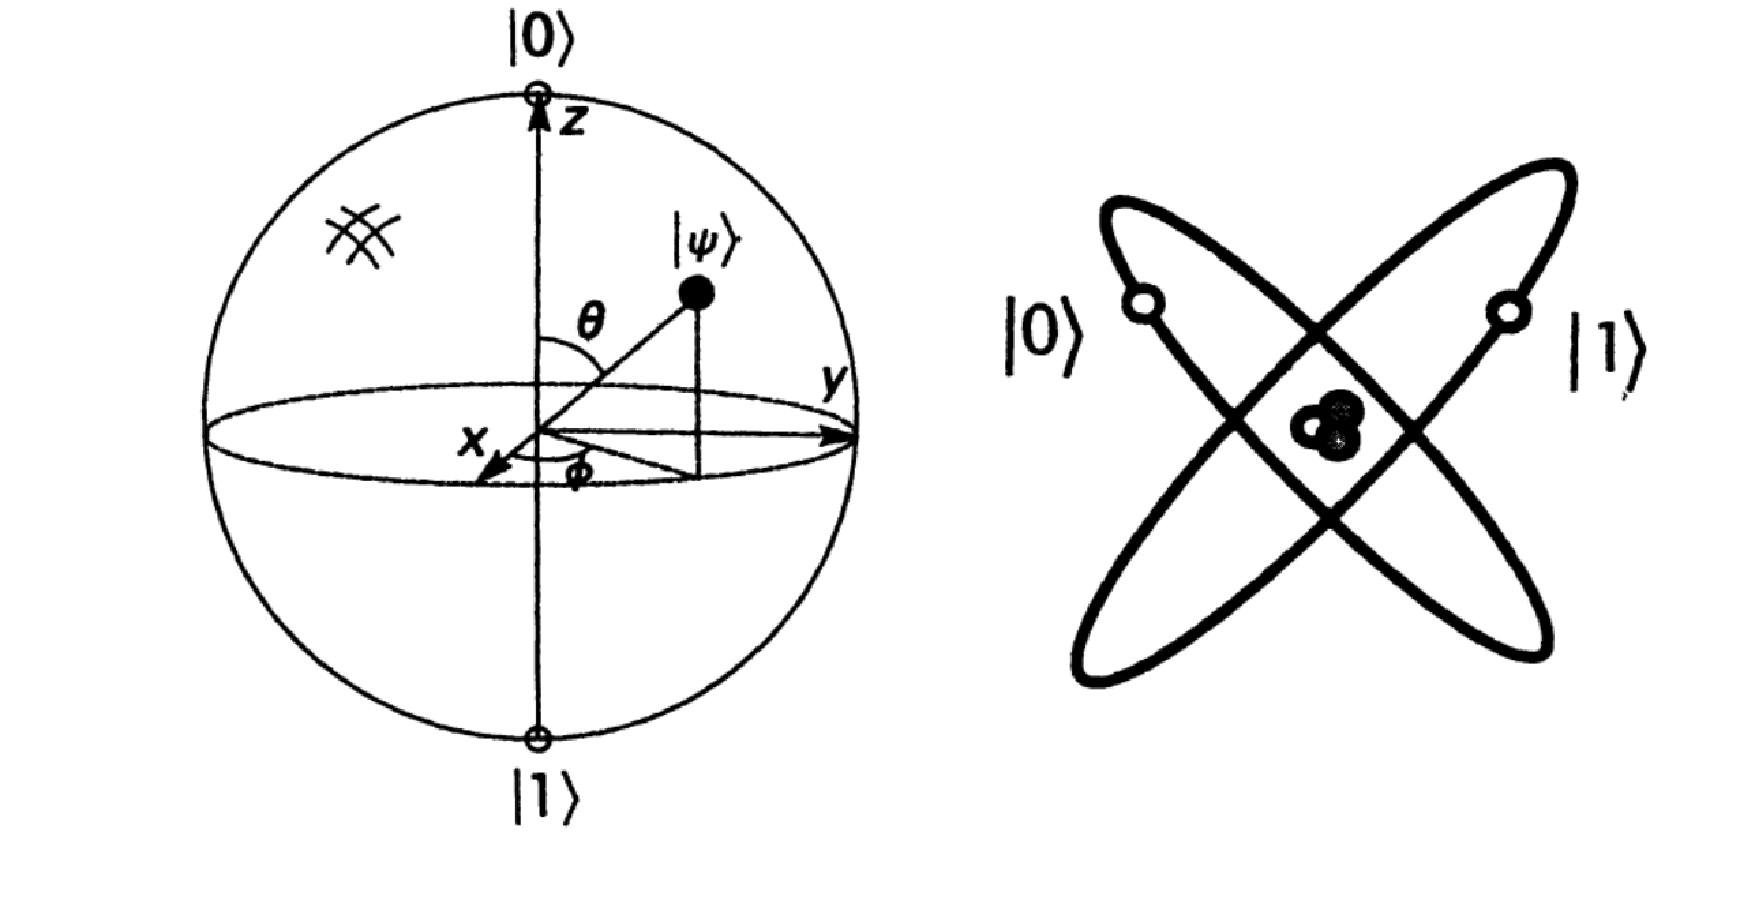
\includegraphics[width=\linewidth]{media/qubits.pdf}
		\end{figure}
	\end{frame}

    \begin{frame}{Захват ионов}
    \framesubtitle{Принцип работы ионной ловушки}

        \begin{columns}

        \begin{column}{1\textwidth}

            \begin{itemize}
                \item По \textit{теореме Ирншоу} заряд не может находится в положении устойчивого равновесия, однако если используя осциллирующие электрические поля можно обойти эту теорему.
                \item Используется линейную ловушку Пола для захвата ионов.
               	\item Получаем уравнение движения в $xy$-плоскости:
               	\begin{equation}
\frac{d^2 x_i}{d \tau^2}=-\frac{4 e V_0}{M r_0^2 \Omega^2} \cos (2 \tau) x_i
\end{equation}
            \end{itemize}

        \end{column}

        %\begin{column}{0.5\textwidth}
        %    \begin{figure}
        %        \centering
        %        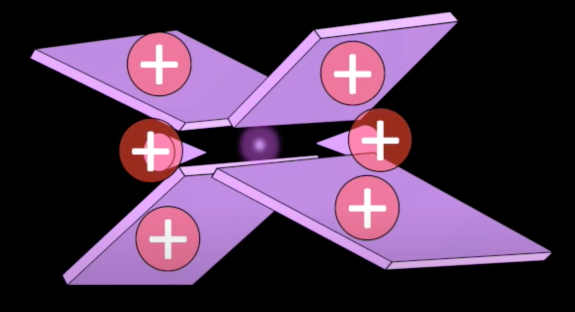
\includegraphics[width=\textwidth]{media/ion-trap.png}
        %        \caption{Схема ионной ловушки}
        %    \end{figure}
        %\end{column}

        \end{columns}

    \end{frame}
		
	
	



    \begin{frame}{Доплеровское охлаждение}
    \framesubtitle{Принцип работы ионной ловушки}

        \begin{columns}

        \begin{column}{0.5\textwidth}

            \begin{itemize}
                \item Стационарный атом не видит лазерного смещения ни в красную, ни в синюю сторону и не поглощает фотон.
                \item Атом, удаляющийся от лазера, видит его сдвиг в красную область и не поглощает фотон.
            
            \end{itemize}

        \end{column}

        \begin{column}{0.5\textwidth}
            \begin{figure}
                \centering
                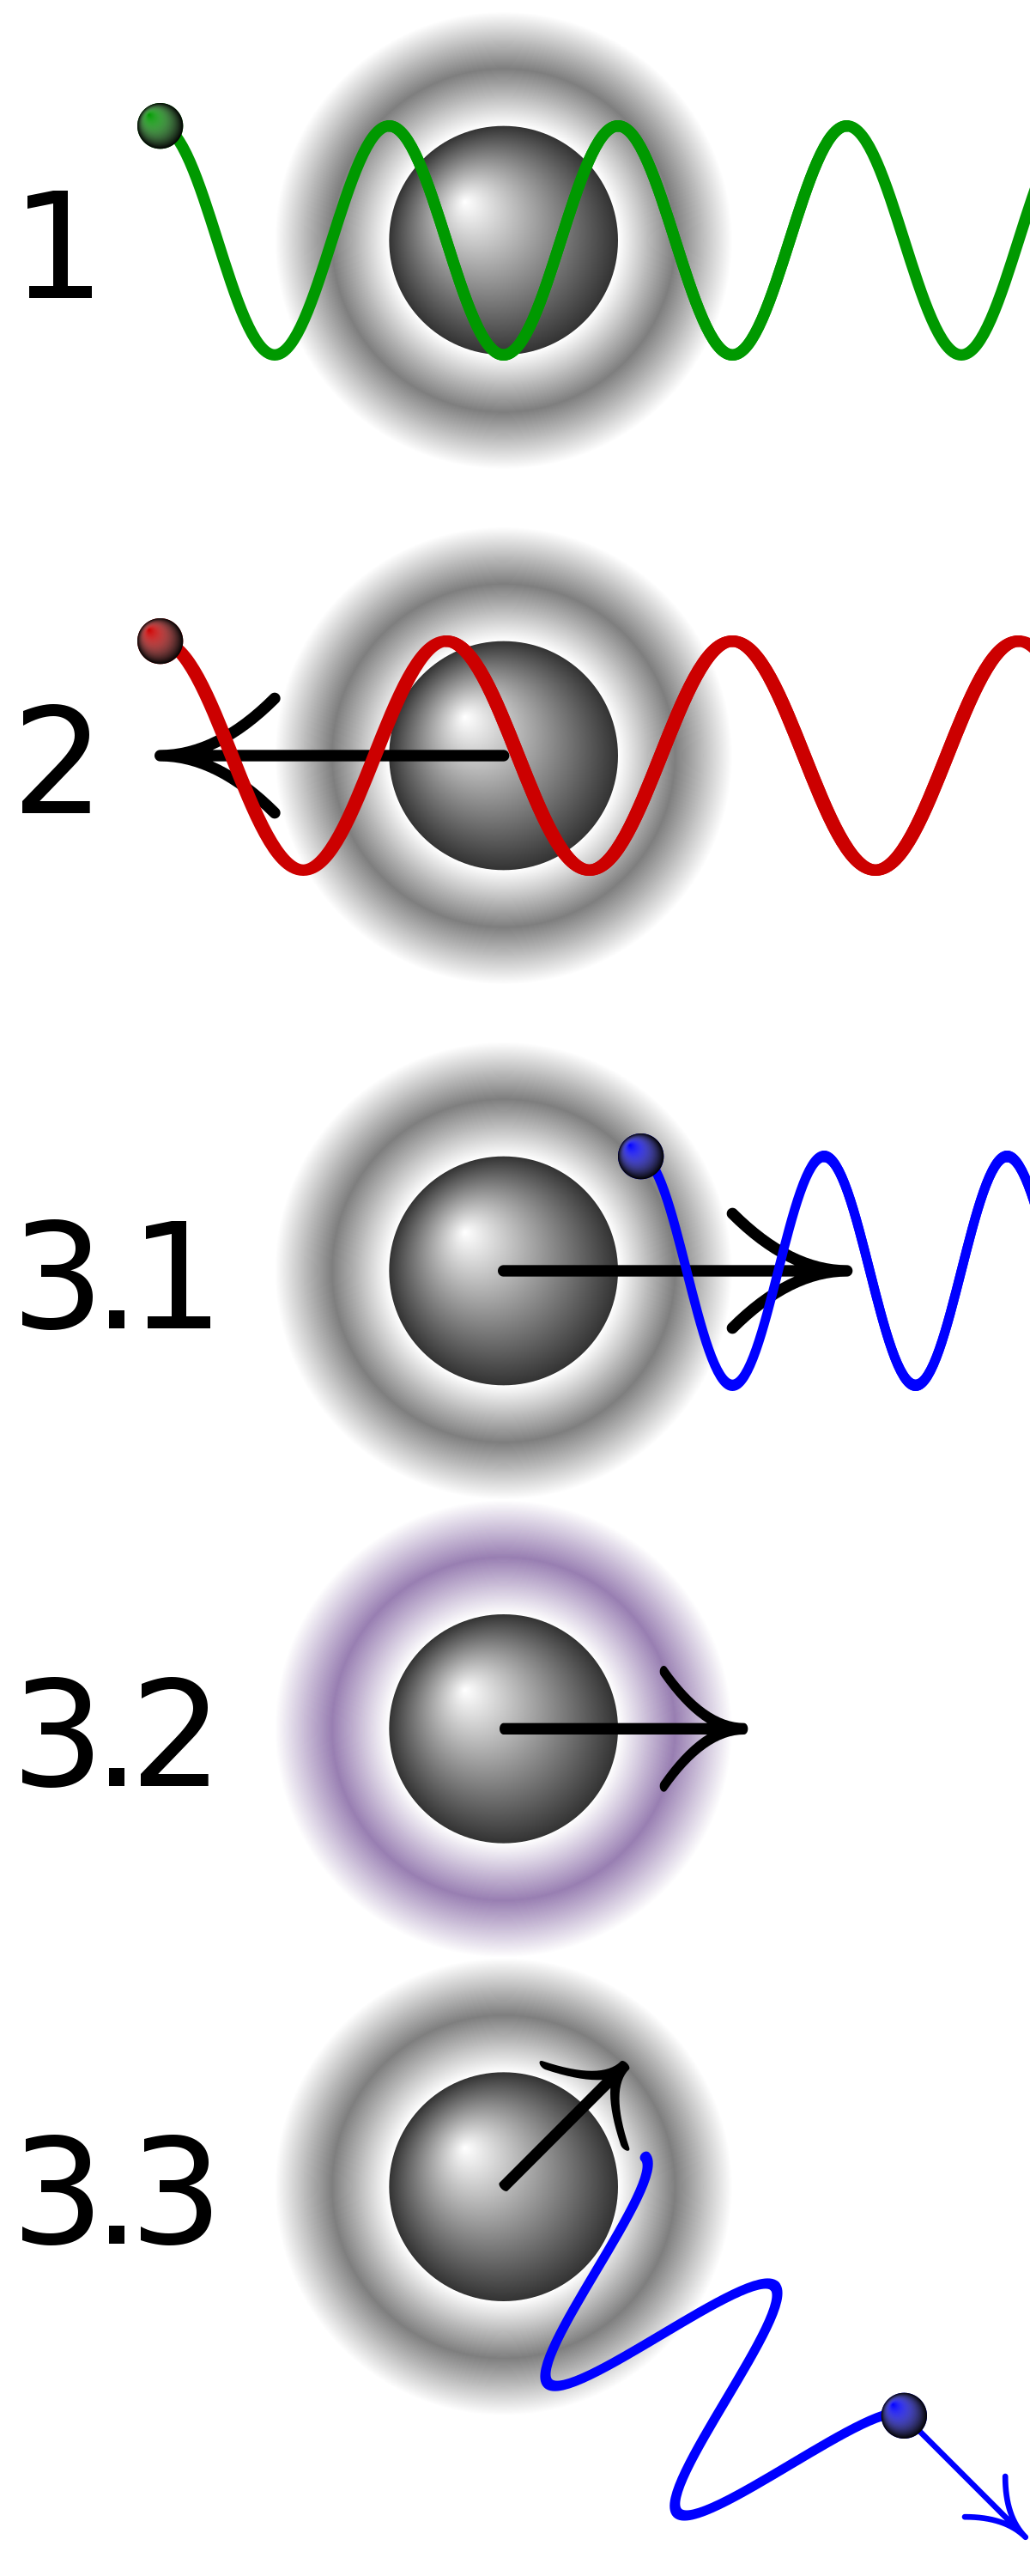
\includegraphics[width=0.35\textwidth]{media/dopler-cooling.png}
                \caption{Иллюстрация доплеровского охлаждения}
            \end{figure}
        \end{column}

        \end{columns}
    \end{frame}

    \begin{frame}{Доплеровское охлаждение}
    \framesubtitle{Принцип работы ионной ловушки}
        \begin{columns}

        \begin{column}{0.5\textwidth}

            \begin{itemize}
            		\item движущийся атом, видит, что он смещен в синий цвет, и поглощает фотон, замедляясь. поглощение фотона.
                \item Фотон возбуждает атом, переводя электрон в более высокое квантовое состояние.
                \item Атом повторно излучает фотон в случайном направлении.
            \end{itemize}

        \end{column}

        \begin{column}{0.5\textwidth}
            \begin{figure}
                \centering
                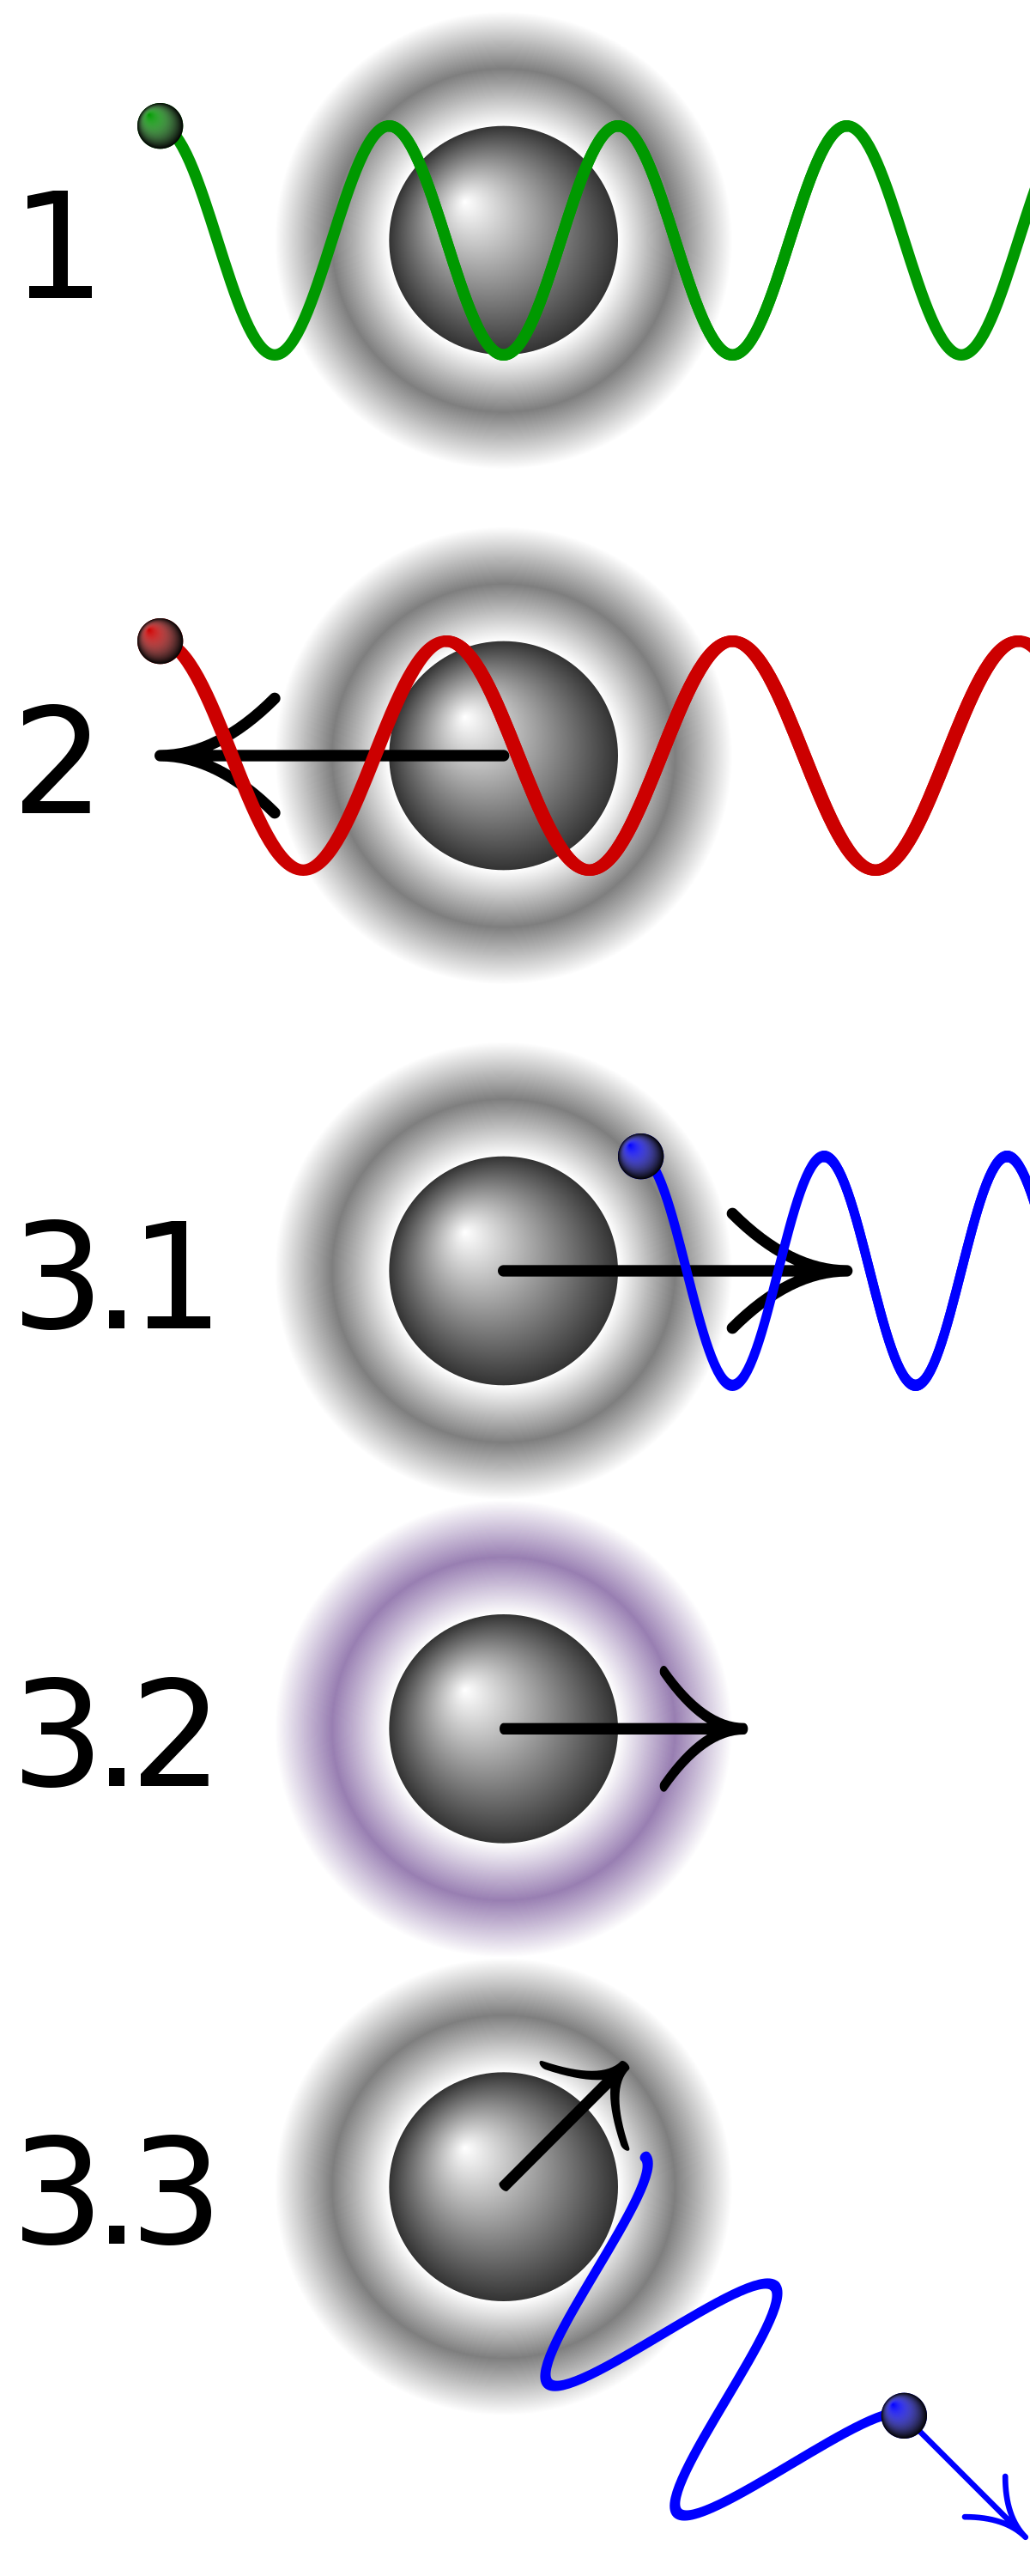
\includegraphics[width=0.35\textwidth]{media/dopler-cooling.png}
                \caption{Иллюстрация доплеровского охлаждения}
            \end{figure}
        \end{column}

        \end{columns}

    \end{frame}


    % \begin{frame}{Захват ионов}
    % \framesubtitle{Принцип работы ионной ловушки}

    %     \movie{\includegraphics[width=\textheight,
    %                      keepaspectratio]
    %                      {media/trapped-ion.jpg}}{media/paul-trap.mp4}

    % \end{frame}

    \begin{frame}{Физическая реализация кубита}
    \framesubtitle{Кубитная ионная ловушка}

        \begin{columns}

        \begin{column}{0.6\textwidth}

            \begin{itemize}
                \item Кубит представляет собой атомные состояния сверхтонкой структуры, удерживаемых в ловушке атомов. 
                \item Два сверхтонких уровня основного состояния (они называются «сверхтонкими кубитами»)
                \item Уровень основного состояния и возбужденный уровень (они называются «оптическими кубитами»)
            \end{itemize}

        \end{column}

        \begin{column}{0.4\textwidth}
            \begin{figure}
                \centering
                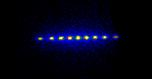
\includegraphics[width=\textwidth]{media/nine-calcium-ions.jpg}
                \caption{Девять атома кальция в ловушке}
            \end{figure}
        \end{column}

        \end{columns}

    \end{frame}
    


    %	\begin{frame}{Физическая реализация кубита}
    %\framesubtitle{Кубитная ионная ловушка}

    %\begin{itemize}
    %        \item Состояния ионных кубитов могут быть приготовлены в определенном состоянии кубита с помощью процесса, называемого \textbf{оптической накачкой}. В этом процессе лазер связывает ион с некоторыми возбужденными состояниями, которые в конечном итоге распадаются до одного состояния, которое не связано с лазером.
    %       \item Как только ион достигает этого состояния, у него нет возбужденных уровней, с которыми можно было бы взаимодействовать в присутствии этого лазера, и, следовательно, он остается в этом состоянии.
    %\end{itemize}


    %\end{frame}

    
    \begin{frame}{Физическая реализация кубита}
    \framesubtitle{Кубитная ионная ловушка}

    \begin{columns}

    \begin{column}{0.5\textwidth}

        \begin{itemize}
                \item Кубит на сверхтонкой структуре - время существование существенно больше времени существования на оптических фотонах.
                \item Можно рассмотреть на примере иона кальция с уровнем $4S_{1/2}$
        \end{itemize}

    \end{column}

    \begin{column}{0.5\textwidth}

        \begin{figure}
            \centering
            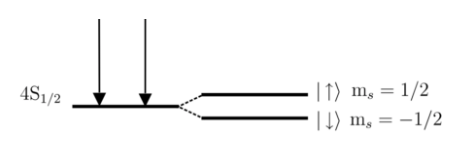
\includegraphics[width=\textwidth]{media/hyperfine-structure.png}
            \caption{Сверхтонкая структура}
        \end{figure}

    \end{column}

    \end{columns}

    \end{frame}

    \begin{frame}{Приготовление начального состояния}
    \framesubtitle{Кубитная ионная ловушка}

    \begin{columns}

    \begin{column}{0.5\textwidth}

        \begin{itemize}
                \item Состояния ионных кубитов могут быть приготовлены в с помощью процесса, называемого \textbf{оптической накачкой}.
        \end{itemize}

    \end{column}

    \begin{column}{0.5\textwidth}

        \begin{figure}
            \centering
            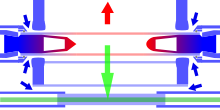
\includegraphics[width=\textwidth]{media/optical-pumping.png}
            \caption{Оптическая накачка лазерного стержня дуговой лампой}
        \end{figure}

    \end{column}

    \end{columns}


    \end{frame}

     \begin{frame}{Приготовление начального состояния}
    \framesubtitle{Кубитная ионная ловушка}

    \begin{columns}

    \begin{column}{0.5\textwidth}

        \begin{itemize}
                \only<1>{\item Рассмотрим энергетические переходы в ионе кальция
                \item Учитывая, что времена жизни должны быть порядка микросекунд
                      для совершения квантовых операций, получим, что некоторые состояния
                      не годятся для выбора в качестве состояния $\ket{1}$}
                \only<2>{\item Например, состояние $3D_{5/2}$ Обладает временем жизни $1.2$ с. Это время жизни годится, так как квантовые операции занимают микросекунды. За время состояние системы не успеет поменяться. }
        \end{itemize}

    \end{column}

    \begin{column}{0.5\textwidth}

        \begin{figure}
            \centering
            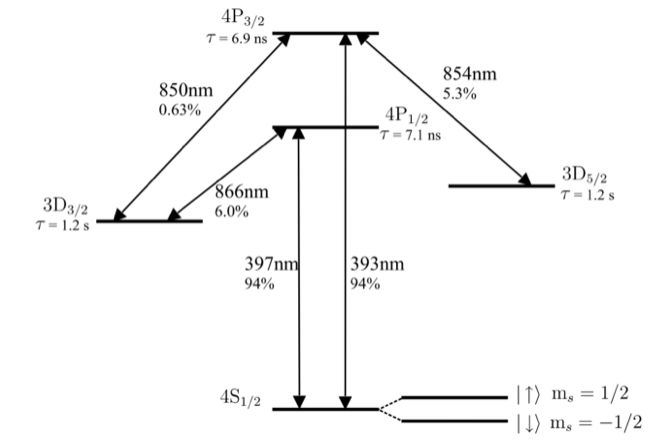
\includegraphics[width=\textwidth]{media/transitions.png}
            \caption{Возможные энергетические переходы}
        \end{figure}

    \end{column}

    \end{columns}

    \end{frame}



    \begin{frame}{Весь процесс приготовления кубита}
    \framesubtitle{Кубитная ионная ловушка}

    \begin{columns}

    \begin{column}{0.5\textwidth}

        \begin{itemize}
                \item Ионизация вещества
                \item Заключение в ионную ловушку
                \item Доплеровское охлаждение
                \item Использование спонтанного и вынужденного излучения для
                      задание состояния иона
        \end{itemize}

    \end{column}

    \begin{column}{0.5\textwidth}

        \begin{figure}
            \centering
            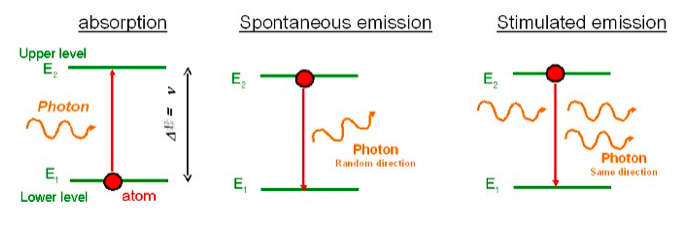
\includegraphics[width=\textwidth]{media/emission-comparison.png}
            \caption{Спонтанное и вынужденное излучение}
        \end{figure}

    \end{column}

    \end{columns}


    \end{frame}


    \begin{frame}{Измерение состояния}
    \framesubtitle{Кубитная ионная ловушкаaa}

        \begin{itemize}

                \item Необходимо воздействовать на ион излучением с частотой перехода с уровня $S$ сверхтонкой структуры на уровень $P$



        \end{itemize}

    \end{frame}

    \begin{frame}{Измерение состояния}
    \framesubtitle{Кубитная ионная ловушкaaа}

    \begin{columns}

    \begin{column}{0.5\textwidth}

        \begin{figure}
            \centering
            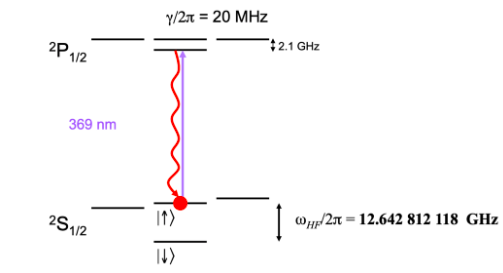
\includegraphics[width=\textwidth]{media/detection1.png}
            \caption{Детектирование состояния 0 (есть излучение)}
        \end{figure}

    \end{column}

    \begin{column}{0.5\textwidth}

        \begin{figure}
            \centering
            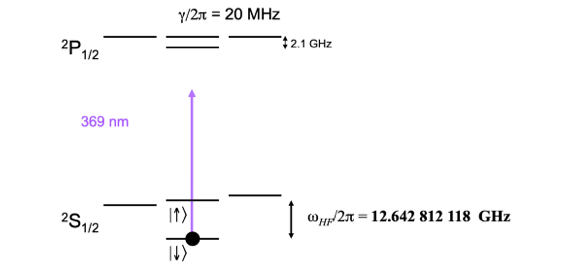
\includegraphics[width=\textwidth]{media/detection2.png}
            \caption{Детектирование состояния 1 (нет излучения)}
        \end{figure}

    \end{column}

    \end{columns}

    \end{frame}

\end{document}
   
